%%%%%%%%%%%%%%%%%%%%%%%%%%%%%%%%%%%%%%%%%%%%%%%%%%%%%%%%%%%%
% Theory book for guitarists
%
%%%%%%%%%%%%%%%%%%%%%%%%%%%%%%%%%%%%%%%%%%%%%%%%%%%%%%%%%%%%

%----------------------------------------------------------------------------------------
%	PACKAGES AND DOCUMENT CONFIGURATIONS
%----------------------------------------------------------------------------------------

\documentclass{article}

% Latex packages
\usepackage{parskip}
\usepackage[shortlabels]{enumitem}
\usepackage{graphicx} % Required for the inclusion of images
\usepackage{amsmath,amssymb} % Required for some math elements
\usepackage{caption}
\usepackage{subcaption}
\usepackage{hyperref}
\setlength\parindent{0pt} % Removes all indentation from paragraphs
\usepackage{booktabs}
\usepackage{changepage}
\usepackage{multirow}
\usepackage{pgfplots} % Include package for TikZ and PGF plot
\usepackage{anyfontsize} % enable to change the font size manually
\usepackage{makecell}%
\usepackage{color}
\usepackage{xcolor}
\usetikzlibrary{shapes.geometric}
\tikzset{
  dot/.style = {circle, fill, minimum size=#1,
                inner sep=0pt, outer sep=0pt},
  dot/.default = 6pt
}


\renewcommand{\labelenumi}{\alph{enumi}.} % Make numbering in the enumerate environment by letter rather than number (e.g. section 6)

%% Recherche des images dans les répertoires.
\graphicspath{{./figures/}{./dia/}{./gnuplot/}}

\title{ Music theory for guitar nerds  } % Title
\author{ Jean-Hughes \textsc{Fournier L.} } % Author name
\date{\today} % Date for the report

\begin{titlepage}
    \centering
	\vspace*{-3cm}
	\hspace*{-5cm}
    \includegraphics[width=22cm]{cover_picture/cover1_original.jpg} % scale as needed
    \vfill
\end{titlepage}


%***********************************************************************************************************************************************
\begin{document}

\maketitle % Insert the title, author and date
\newpage
\tableofcontents
\newpage

\begin{itemize}
	\item Gives the recipe not just examples
	\item If you give a man a fish, you feed him for a day. If you teach a man to fish, you feed him for a lifetime
\end{itemize}

%%%%%%%%%%%%%%%%%%%%%%%%%%%%%%%%%%%%%%%%%%%%%%%%%%%%%%%%%%%%%%%%%%%%%%%%%%%%%%%%%%%%%%%%%%%%%%%%%%%%%%%%%%%%%%%%%%%%%
\section{Intervals: where do notes come from?}
%%%%%%%%%%%%%%%%%%%%%%%%%%%%%%%%%%%%%%%%%%%%%%%%%%%%%%%%%%%%%%%%%%%%%%%%%%%%%%%%%%%%%%%%%%%%%%%%%%%%%%%%%%%%%%%%%%%%%

%Names of the interval comes from the diatonic scale. In C major scale (C-D-E-F-G-A-B-C) that scale G$\#$ is the augmented 5. In C minor scale (C-D-Eb-F-G-Ab-Bb) G$\#$ is the minor sixth.

\subsection{Harmonic series}

% Figure
\begin{figure}[h!]
	\centering
%	\hspace*{0cm}
	\scalebox{1}{\input{figures/1.intervalles/serie_harmonique.tex}}
	\caption{The harmonic series}
	\label{fig:serie_harmonique}
\end{figure}

\subsection{Intervals definition}
% Table

% Table
\begin{table*}[!h]
	\caption{Intervals and }
	\centering
	\begin{tabular}{|c|c|c|c|c|c|c|c|}
		\hline 
		\multicolumn{5}{|c|}{\textbf{Harmonics}}  &  \textbf{Ratio to fundamental} & \textbf{Intervals}  & \textbf{Equal Temperament}  \\
		\hline
		1 & 2 & 4 & 8 & 16  & 1,2,3,4 & unison/octave      & 1.000 \\
		\hline
		  &   &   &   & 17  & $17/16=1.0625$ & minor second & 1.059 \\
		  \hline
		  &   &   & 9 & 18   & $9/8=1.125$ & major second  & 1.122 \\
		  \hline
		  &   &   &   & 19    & $19/16=1.1875$ & minor third  & 1.189 \\
		  \hline
		  &   & 5 &10 & 20    & $5/4=1.2500$ & major third & 1.260 \\
		  \hline
		  &   &   &   & 21   & $21/16=1.3125$ & fourth & 1.335 \\
		  \hline
		  &   &   & 11& 22  & $11/8=1.375$ & \multirow{2}{*}{tritone}  & \multirow{2}{*}{$1.414$} \\
		  &   &   &   & 23  & $23/16=1.4375$ &   &  \\
		  \hline
		  & 3 & 6 &12 & 24 & $3/2=1.500$ &  fifth  & 1.498 \\
		  \hline
		  &   &   &  & 25 & $25/16=1.5625$ & \multirow{2}{*}{minor sixth} &\multirow{2}{*}{$1.587$}\\
		  &   &   &13 & 26 & $13/8 = 1.625$              &             &  \\
		  \hline
		  &   &   &   & 27    & $27/16=1.6875$ & major sixth & 1.682 \\
		  \hline
		  &   & 7 & 14& 28 & $7/4=1.7500$ & \multirow{2}{*}{minor seventh} & \multirow{2}{*}{$1.782$}  \\
		  &   &   &   & 29 & $29/16 = 1.8125$         &             &  \\
		  \hline
		  &   &   & 15& 30 & $15/8=1.875$ & \multirow{2}{*}{major seventh} & \multirow{2}{*}{$1.888$} \\
		  &   &   &   & 31 & $31/16=1.9375$        &  &  \\
		\hline
	\end{tabular}
	\label{tab: }
\end{table*}



 Table
 Source: https://hellomusictheory.com/learn/intervals/
\begin{table*}[!h]
	\caption{Intervals chart in relation to C note. Minor (m or ``-''), major (M or ``maj''), augmented (A or ``aug'' or ``$\#$'' or ``$+$'') and diminished (d or ``dim'' or ``b''). }
	\centering
	\begin{adjustwidth}{-2cm}{}
	\begin{tabular}{clccl}
		\hline 
		\textbf{Semitones} & \textbf{Name} & \textbf{Notation} & \textbf{notation} & \textbf{Songs}  \\
		\hline
		0 & Perfect unison            & P1 & C & -   \\
		\hline
		1 & Minor second              & m2 & b2 & JAWS theme \\
		2 & Major second              & M2 & 2 & \textbf{Frè-re} Jacques  \\
		\hline
		3 & Minor third               & m3 & b3 & Iron Man by Black Sabbath\\
		4 & Major third               & M3 & 3 & "\textbf{Oh-When} the Saints" \\
		\hline
		5 & Perfect fourth            & P4 & 4 & Here Comes the Bride (Wedding song) \\
		\hline
		6 & Triton                    & T  & b5 & "\textbf{The - Simp}-sons" \\
		\hline
		7 & Perfect fifth             & P5 &  5 &"\textbf{Twinkle - Twinkle} Little Star"   \\
		\hline
		8 & Minor sixth               & m6 &  b6 & The Entertainer \\
		9 & Major sixth               & M6 &  6 & Jingle Bells ("\textbf{Dash-ing} through the snow")   \\
		\hline
		10 & Minor seventh            & m7 &  b7 & Theme song Star Trek : The Original Series\\
		11 & Major seventh            & M7 &  7 & Take On Me ("Take-on")  \\
		\hline
		12 & Perfect octave           & P8 &  8 & "\textbf{Some-where} over the rainbow" \\
		\hline
		13 & Minor ninth              & m9 &  b9 \\
		14 & Major ninth              & M9 &  9 \\
		15 & Augmented ninth          & A9 &  $\#$9 \\
		\hline
		16 & Diminished eleventh      & d11 & b11 \\
		17 & Perfect eleventh         & P11 & 11 \\
		18 & Augmented eleventh       & A11 & $\#$$11 \\
		\hline
		20 & Minor thirteenth         & m13 & b13 \\
		21 & Major thirteenth         & M13 & 13 \\
		\hline
	\end{tabular}
	\end{adjustwidth}
	\label{tab: }
\end{table*}


% ****************************************************************************
\subsection{Consonance and dissonance}

% Figure
\begin{figure}[h!]
	\centering
	\hspace*{0cm}
	\includegraphics[scale=0.03, trim= {0cm 0cm 0cm 0cm}, clip]{figures/1.intervalles/Harmonic_entropy.png}
	\caption{Harmonic entropy}
	\label{fig:harmonic_entro}
\end{figure}

% Figure
\begin{figure}[h!]
	\centering
	\hspace*{0cm}
	\includegraphics[scale=0.5, trim= {0cm 0cm 0cm 0cm}, clip]{figures/1.intervalles/battement/main.pdf}
%	\scalebox{0.3}{\documentclass{standalone}
\usepackage{pgfplots} % Include package for TikZ and PGF plot
\usepackage{anyfontsize} % enable to change the font size manually 
\usepackage{makecell}%
\usetikzlibrary{shapes.geometric}
\tikzset{
dot/.style = {circle, fill, minimum size=#1,
              inner sep=0pt, outer sep=0pt},
dot/.default = 6pt % size of the circle diameter 
}
 \renewcommand{\familydefault}{\sfdefault}

\begin{document}
\begin{tikzpicture}[scale=1]
	\def \R{10cm}
	
	
	\draw[black, thick] (0,0) circle (\R); 
	\draw[black, thick] (0,0) circle (2*\R/3); 
	
	
	\node[] at (0,8cm) {{\large C}};
	
	%\fill[black, line width=2] (0.0,-0.4) rectangle (20*\fret,4.4);
	%\draw[color=black!50!white, thick]  (0, 0)   -- (0,5*\h); 
	
	
\end{tikzpicture}
\end{document}}
	\caption{Beat tone}
	\label{fig:battement}
\end{figure}


\clearpage
%%%%%%%%%%%%%%%%%%%%%%%%%%%%%%%%%%%%%%%%%%%%%%%%%%%%%%%%%%%%%%%%%%%%%%%%%%%%%%%%%%%%%%%%%%%%%%%%%%%%%%%%%%%%%%%%%%%%%
% Interval of notes create scales
\section{Scales}
%%%%%%%%%%%%%%%%%%%%%%%%%%%%%%%%%%%%%%%%%%%%%%%%%%%%%%%%%%%%%%%%%%%%%%%%%%%%%%%%%%%%%%%%%%%%%%%%%%%%%%%%%%%%%%%%%%%%%

% Table

\begin{table*}[!h]
	\caption{Scales formula (relative to the major scale)}
	\begin{adjustwidth}{-2.5cm}{}
	\begin{tabular}{l|ccc cccc|l}
		Scale name  & \multicolumn{7}{c}{Formula} & Comment \\ 
		\hline \hline \vspace{-0.4cm} \\
		\textcolor{yellow!90!black}{Major} & \textcolor{yellow!90!black}{1}  
										    & \textcolor{yellow!90!black}{2}  
										    & \textcolor{yellow!90!black}{3}  
										    & \textcolor{yellow!90!black}{4} 
										    & \textcolor{yellow!90!black}{5}  
										    & \textcolor{yellow!90!black}{6} 
										    & \textcolor{yellow!90!black}{7} & \\
		\textcolor{red!60!white}{Natural minor}      & \textcolor{red!60!white}{1} 
													  & \textcolor{red!60!white}{2} 
													  & \textcolor{red!60!white}{b3} 
													  & \textcolor{red!60!white}{4}      
													  & \textcolor{red!60!white}{5}   
													  & \textcolor{red!60!white}{b6} 
													  & \textcolor{red!60!white}{b7} 
													  & \\
		Harmonic minor          & 1 & 2  & b3 & 4  & 5  & b6 & \textcolor{black}{\fbox{7}}  &  \\
		Melodic minor           & 1 & 2  & b3 & 4  & 5  & \textcolor{black}{\fbox{6}}  & 7  &  \\ 
		Pentatonic Major   & 1 & 2  & 3  &   -   & 5  & 6  &  - &  \\
		Pentatonic minor        & 1 &  - & b3 & 4  & 5  & - &  b7 &  \\
		\hline
		
		\textcolor{yellow!90!black}{Ionian (Major)}  & \textcolor{yellow!90!black}{1}  
											  		  & \textcolor{yellow!90!black}{2}  
											  		  & \textcolor{yellow!90!black}{3}  
											  		  & \textcolor{yellow!90!black}{4} 
											  		  & \textcolor{yellow!90!black}{5}  
											  		  & \textcolor{yellow!90!black}{6} 
											  		  & \textcolor{yellow!90!black}{7} & \\ 
		\textcolor{green!60!white!70!black}{Dorian}  & \textcolor{green!60!white!70!black}{1} 
													  & \textcolor{green!60!white!70!black}{2} 
													  & \textcolor{green!60!white!70!black}{b3} 
													  & \textcolor{green!60!white!70!black}{4} 
													  & \textcolor{green!60!white!70!black}{5}  
													  & \textcolor{green!60!white!70!black}{\fbox{6} }
													  & \textcolor{green!60!white!70!black}{b7} & Mad world, So What \\ 
		\textcolor{cyan}{Phrygian}                   & \textcolor{cyan}{1} 
													  & \textcolor{cyan}{\fbox{b2}}
													  & \textcolor{cyan}{b3} 
													  & \textcolor{cyan}{4} 
													  & \textcolor{cyan}{5}  
													  & \textcolor{cyan}{b6} 
													  & \textcolor{cyan}{b7} & Symphony of destruction\\ 
		\textcolor{blue!50!white}{Lydian}            & \textcolor{blue!50!white}{1} 
													  & \textcolor{blue!50!white}{2}
													  & \textcolor{blue!50!white}{3}  
													  & \textcolor{blue!50!white}{\fbox{$\#$4}}
													  & \textcolor{blue!50!white}{5}  
													  & \textcolor{blue!50!white}{6}  
													  & \textcolor{blue!50!white}{7}  
													  &  Legend of Zelda\\ 
		\textcolor{blue!50!red!50!white}{Mixolydian} & \textcolor{blue!50!red!50!white}{1} 
													  & \textcolor{blue!50!red!50!white}{2} 
													  & \textcolor{blue!50!red!50!white}{3} 
													  & \textcolor{blue!50!red!50!white}{4}    
													  & \textcolor{blue!50!red!50!white}{5}
													  & \textcolor{blue!50!red!50!white}{6}
													  & \textcolor{blue!50!red!50!white}{\fbox{b7}}
													  & Clock by Coldplay\\ 
		\textcolor{red!60!white}{Aeolian (natural minor)} & \textcolor{red!60!white}{1} 
													  & \textcolor{red!60!white}{2} 
													  & \textcolor{red!60!white}{b3} 
													  & \textcolor{red!60!white}{4}      
													  & \textcolor{red!60!white}{5}   
													  & \textcolor{red!60!white}{b6} 
													  & \textcolor{red!60!white}{b7} 
													  & Smell Like Teen Spirit\\
		\textcolor{orange!80!white}{Locrian}         & \textcolor{orange!80!white}{1}
													  & \textcolor{orange!80!white}{b2} 
													  & \textcolor{orange!80!white}{b3}
													  & \textcolor{orange!80!white}{4}   
													  & \textcolor{orange!80!white}{\fbox{b5}}
													  & \textcolor{orange!80!white}{b6}
													  & \textcolor{orange!80!white}{b7}
													  & Rush-YYZ intro\\ 
		
		\hline 
		\textcolor{yellow!90!black}{Ionian b6}    & \textcolor{yellow!90!black}{1} 
												   & \textcolor{yellow!90!black}{2}
												   & \textcolor{yellow!90!black}{3}
												   & \textcolor{yellow!90!black}{4}
												   & \textcolor{yellow!90!black}{5}
												   & \textcolor{yellow!90!black}{\textcolor{yellow!90!black}{b6}}
												   & \textcolor{yellow!90!black}{7}\\ 
		\textcolor{green!60!white!70!black}{Dorian {\footnotesize $\#$}4} (4$^{\textrm{th}}$ Harm. min) & \textcolor{green!60!white!70!black}{1} 
																							& \textcolor{green!60!white!70!black}{2}  
																							& \textcolor{green!60!white!70!black}{b3} 
																							& \textcolor{green!60!white!70!black}{\textcolor{green!60!white!70!black}{{\footnotesize $\#$}4}}
																							& \textcolor{green!60!white!70!black}{5}  
																							& \textcolor{green!60!white!70!black}{6}  
																							& \textcolor{green!60!white!70!black}{b7} 
																						    & Klezmer music (Jewish)\\
		\textcolor{cyan}{Phrygian dominant} (5th Harm. min) & \textcolor{cyan}{1} 
													  & \textcolor{cyan}{b2} 
													  & \textcolor{cyan}{\textcolor{cyan}{3}}
													  & \textcolor{cyan}{4} 
													  & \textcolor{cyan}{5}  
													  & \textcolor{cyan}{b6} 
													  & \textcolor{cyan}{b7} & Flamenco, \textit{Come out and play} \\
		\textcolor{blue!50!white}{Lydian dominant} (4th Melo. min)  & \textcolor{blue!50!white}{1} 
																	  & \textcolor{blue!50!white}{2}
																	  & \textcolor{blue!50!white}{3} 
																	  & \textcolor{blue!50!white}{{\footnotesize $\#$}4 }
																	  & \textcolor{blue!50!white}{5}
																	  & \textcolor{blue!50!white}{6} 
																	  & \textcolor{blue!50!white}{\textcolor{blue!50!white}{b7}}
																	  & Prog futuristic, Simpsons theme\\  
		\textcolor{blue!50!red!50!white}{Mixolydian b6} (5th Melo. min)  & \textcolor{blue!50!red!50!white}{1} 
																		   & \textcolor{blue!50!red!50!white}{2}  
																		   & \textcolor{blue!50!red!50!white}{\textcolor{blue!50!red!50!white}{3} }
																		   & \textcolor{blue!50!red!50!white}{4}
																		   & \textcolor{blue!50!red!50!white}{5} 
																		   & \textcolor{blue!50!red!50!white}{b6}  
																		   & \textcolor{blue!50!red!50!white}{b7} 
																		   & Prog rock \\
		(or Aeolian dominant) & & & &   & & & &\\
		Neapolitan minor                   & \textcolor{black}{1} 
													  & \textcolor{black}{b2} 
													  & \textcolor{black}{b3} 
													  & \textcolor{black}{4} 
													  & \textcolor{black}{5}  
													  & \textcolor{black}{b6} 
													  & \textcolor{black}{7} &\\                                                                                
		\hline 
		Bizantine scale (double harmonic major)      & \textcolor{black}{1} 
													  & \textcolor{black}{b2} 
													  & \textcolor{black}{3} 
													  & \textcolor{black}{4} 
													  & \textcolor{black}{5}  
													  & \textcolor{black}{b6} 
													  & \textcolor{black}{7} & Opeth - Bleak\\
	    Lydian $\#$2,$\#$6                           & & & & & & & \\
	    Ultra-Phrygian                               &1 &b2 &b3 &b4 &5 &b6 &bb7 \\
		Hungarian minor (double harmonic minor)      & \textcolor{black}{1} 
													  & \textcolor{black}{2} 
													  & \textcolor{black}{b3} 
													  & \textcolor{black}{$\#$4} 
													  & \textcolor{black}{5}  
													  & \textcolor{black}{b6} 
													  & \textcolor{black}{7} & \\ 
	    Oriental (Asian)                             & & & & & & & \\
	    Ionian Aug$\#$2                             & 1&$\#$2 &3 &4 &$\#$5 &6 &7 \\
	    Locrian bb3,bb7                             & 1 &b2 &bb3 &4 &b5 &b6 &bb7 \\
		\hline 
	\end{tabular}
	\label{tab: }
	\end{adjustwidth}
\end{table*}



\clearpage
% #################################################
\subsection{Major scale fretboard positions}

% Figure: gamme majeur pattern sur manche
\begin{figure}[h!]
	\centering
	\hspace*{-2cm}
%	\includegraphics[scale=0.55, trim= {0cm 0cm 0cm 0cm}, clip]{gamme_majeure_manche/main.pdf}
%	\scalebox{0.5}{\input{figures/2.gammes/gamme_majeure_manche.tex}}
%	\hspace*{-2cm}
	\scalebox{0.5}{\input{figures/2.gammes/gamme_majeure/pos1.tex}}
	\hspace*{-2cm}
	\scalebox{0.5}{\input{figures/2.gammes/gamme_majeure/pos2.tex}}
	\hspace*{-2cm}
	\scalebox{0.5}{\input{figures/2.gammes/gamme_majeure/pos3.tex}}
	\hspace*{-2cm}
	\scalebox{0.5}{\input{figures/2.gammes/gamme_majeure/pos4.tex}}
	\hspace*{-2cm}
	\scalebox{0.5}{\input{figures/2.gammes/gamme_majeure/pos5.tex}}
	\caption{G Major scale on the fretboard position 1, 2, 3, 4 and 5.}
	\label{fig:gamme_majeure_manche}
\end{figure}

% #################################################
\clearpage
\subsection{Pentatonic scale on the fretboard}

% Figure: gamme penta pattern sur manche
\begin{figure}[h!]
	\centering
%	\hspace*{-2cm}
%	\scalebox{0.5}{\input{figures/2.gammes/gamme_penta/gamme_penta_manche.tex}}
	\hspace*{-2cm}
	\scalebox{0.5}{\input{figures/2.gammes/gamme_penta/pos1.tex}}
	\hspace*{-2cm}
	\scalebox{0.5}{\input{figures/2.gammes/gamme_penta/pos2.tex}}
	\hspace*{-2cm}
	\scalebox{0.5}{\input{figures/2.gammes/gamme_penta/pos3.tex}}
	\hspace*{-2cm}
	\scalebox{0.5}{\input{figures/2.gammes/gamme_penta/pos4.tex}}
	\hspace*{-2cm}
	\scalebox{0.5}{\input{figures/2.gammes/gamme_penta/pos5.tex}}
	\caption{Pattern of pentatonic scales}
	\label{fig:gammme_penta_manche}
\end{figure}

% #################################################
\subsection{Minor melodic scale}

\subsection{Minor harmonic scale}

\subsection{Diminished scale}
\begin{figure}[h!]
	\centering
	\hspace*{-2cm}
	\scalebox{0.5}{\input{figures/2.gammes/gamme_diminue/pos1.tex}}
	\hspace*{-2cm}
	\scalebox{0.5}{\input{figures/2.gammes/gamme_diminue/pos2.tex}}
	\caption{G diminished scales with two fingering. }
	\label{fig:gammme_diminue}
\end{figure}


%%%%%%%%%%%%%%%%%%%%%%%%%%%%%%%%%%%%%%%%%%%%%%%%%%%%%%%%%%%%%%%%%%
% Construction of chords superimposing 3rds on a scale
\clearpage
\section{Chords}
%%%%%%%%%%%%%%%%%%%%%%%%%%%%%%%%%%%%%%%%%%%%%%%%%%%%%%%%%%%%%%%%%%%%%%%

\begin{itemize}
	\item Tonic: I, iii, vi
	\item Pre-dominant: IV, ii
	\item Dominant: V, vii$^\circ$
\end{itemize}


\begin{itemize}
	\item ``Sus'' chords: chord without third
	\item ``sus9'' will often replace the dominant 7th chord
\end{itemize}

%%%%%%%%%%%%%%%%%%%%%%%%%%%%%%%%%%%%%%%%%%%%%%%%%%%%%%%%%%%%%%%%%%%%%%%%%%%%%%%%%%%%%%%%%%%%%%%%%%%%%%%%%
\clearpage
\subsection{Formation of chords}

% Table
% Source: 1997 - Vaillot Méthode Jazz
% Tetrad: https://www.beyondmusictheory.org/chord-formations-triads-and-tetrads/
% Nom de acccords Jake lizzio
\usepackage{arydshln}


\begin{table*}[!h]
	\centering
	\caption{Construction of chords (notation is relative to the major scale)}
	\begin{tabular}{clccclcccl}
		\hline \vspace{-0.2cm} \\
		 & chord & symbol & & & & & & & name \\
		\hline \vspace{-0.2cm} \\
		\multirow{4}{*}{triad} &         & & 1 & 3 & 5           & & & & major\\
		                       & m       & & 1 & b3 & 5           & & & & minor\\
		                       & dim     & $^\circ$ & 1 & b3 & b5     & & & & diminished\\
		                       & aug     & + & 1 & 3 & $^\#$5 & & & & augmented \\
		\hline  \vspace{-0.2cm} \\
		\multirow{4}{*}{ }    & sus2     & & 1 & 2  & 5   &   &   & & suspended 2nd \\
		                       & sus4    & & 1 & 4   & 5   &   &   & & suspended 4th \\
		\hline \vspace{-0.2cm} \\
		\multirow{8}{*}{tetrad}& 7       &               & 1 & 3  & 5 & b7                & & & dominant 7th \\
		                       & maj7   & $\Delta$, M$7$      & 1 & 3  & 5 & 7  & & & major 7th\\
		                       & m7     & $^{-}$7        & 1 & b3  & 5 & b7  & & & minor 7th\\
		                       & m7b5   & $\varnothing$            & 1 & b3  & b5 & b7 & & & half-diminished \\
		                       & dim7   & $^{\circ}$7        & 1 & b3  & b5 & b7  & & & fully-diminished\\
        					   & mM7    & m$^\Delta$          & 1 & b3  & 5 & 7   & & & minor major 7th \\
							   & maj7($\#$5) & $+^{\Delta}$    & 1 & 3  & $\#$5 & 7  & & & augmented major 7th \\
		                       & 7($\#$5)    & $+^{7}$    & 1 & 3  & $\#$5 & b7  & & & augmented 7th \\
		\hline \vspace{-0.2cm} \\
							   & 6       & & 1 & 3  & 5 & 6   &   & \\
                               & m6      & & 1 & b3  & 5 & 6   &   & \\
							   & b6      & & 1 & 3  & 5 & b6   &   & \\
                               & m(b6)   & & 1 & b3  & 5 & b6   &   & \\
		                       & m6/9    & & 1 & b3  & 6 & 9  &   & \\
		                       & 6/9     & & 1 & 3  & 6 & 9  &   & \\
		                       & add9    & & 1 & 3  & 5 & 9  &   & \\
		  					   & m(add9) & & 1 & b3  & 5 & 9  &   & \\
		\hline  \vspace{-0.2cm} \\
							   & 7sus4   & & 1 & 4   & 5 & b7  &  & \\
		                       & add2    & & 1 & 2  & 3 & 5   &  & \\
		\hline
		\multirow{4}{*}{pentad}& 9     & & 1 & 3  & 5 & b7  & 9  & & Dominant 9th \\
	                           & maj9  &$\Delta9$  & 1 & 3  & 5 & 7  & 9  & & major 9th \\
		                       & 7b9 & & 1 & 3  & 5 & b7  & b9  &\\
		                       & m9    & & 1 & b3  & 5 & b7  & 9  & & minor 9th \\
							   & mM9    & & 1 & b3  & 5 & 7  & 9  & & minor major 9th\\
		\hline  \vspace{-0.2cm} \\
		                       & sus9  & & 1 & 4   & 5 & b7  & 9  & \\
		                       & 11    & & 1 & 5   & b7 & 9  & 11  & \\ % The 3 is omitted to avoid the dissonace between 3-11.
		\hline
		\multirow{2}{*}{hexad} & 7(13)     & & 1 & 3  & 5 & b7  & 9  & 13\\ % the 11 is omited to avoid the dissonance between 3-11.
		                       & 7(b9,13)  & & 1 & 3  & 5 & b7  & b9  & 13\\
		\hline \vspace{-0.2cm}
	\end{tabular}
	\label{tab: }
\end{table*}

- Accords: 7, m7, maj7, m7b5 (root sur corde E, A, D)


\clearpage
\subsection{Diatonic chords}
% Table
\input{figures/3.accords/table-diatonic_chords}

% Table
\input{figures/3.accords/table-modes.tex}

\subsection{Extended chords}

https://music.stackexchange.com/questions/108060/extended-chord-types-for-all-major-scale-degrees

%%%%%%%%%%%%%%%%%%%%%%%%%%%%%%%%%%%%%%%%%%%%%%%%%%%%%%%%%%%%%%%%%%%%%%%%%%%%%%%%%%%%%%%%%%%%%%%%%%%%%%%%%
\clearpage
\subsection{Chord inversions}

% Figure
\begin{figure}[h!]
	\centering
	\hspace*{-2.2cm}
	\scalebox{0.7}{\input{figures/3.accords/chord-inversions/maj7.tex}}
	\hspace*{-2.2cm}
	\scalebox{0.7}{\input{figures/3.accords/chord-inversions/Dom7.tex}}
	\hspace*{-2.2cm}
	\scalebox{0.7}{\input{figures/3.accords/chord-inversions/m7.tex}}
	\hspace*{-2.2cm}
	\scalebox{0.7}{
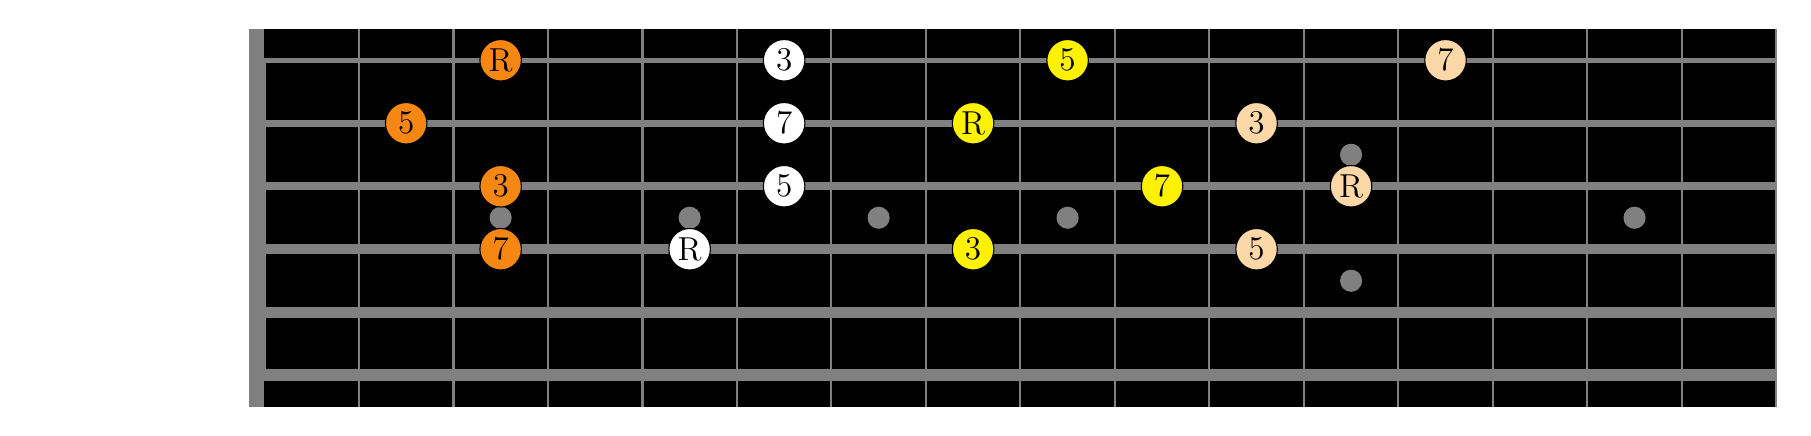
\begin{tikzpicture}[scale=1]
	\def \h{0.8}
	\def \fret{1.2} % 1.6
	\def \L{ 16*\fret }	
	\def \dot_size{4pt}
	\def \circ_size{15pt}
	
	\fill[black, line width=2] (0.0,-0.4) rectangle (16*\fret,4.4);
	\fill[black!50!white, line width=2] (-0.2,-0.4) rectangle (0,4.4);
	
	% Strings
	\draw[color=black!50!white, line width=2.0]  (-0.1, 5*\h) -- (\L,5*\h); % E
	\draw[color=black!50!white, line width=2.5]  (-0.1, 4*\h) -- (\L,4*\h); % B
	\draw[color=black!50!white, line width=3.0]  (-0.1, 3*\h) -- (\L,3*\h); % G
	\draw[color=black!50!white, line width=3.5]  (-0.1, 2*\h) -- (\L,2*\h); % D
	\draw[color=black!50!white, line width=4.0]  (-0.1, 1*\h) -- (\L,1*\h); % A
	\draw[color=black!50!white, line width=4.5]  (-0.1, 0*\h) -- (\L,0*\h); % E
	
	% Frets 0
	\draw[color=black!50!white, thick]  (-0.1, 0) -- (-0.1,5*\h); 
	\draw[color=black!50!white, thick]  (0, 0)   -- (0,5*\h); 
	
	% Fret 1-15
	\draw[color=black!50!white, thick]  (\fret,   -0.4)   -- (\fret,4.4);   
	\draw[color=black!50!white, thick]  (2*\fret, -0.4) -- (2*\fret,4.4); 
	\draw[color=black!50!white, thick]  (3*\fret, -0.4) -- (3*\fret,4.4); 
	\draw[color=black!50!white, thick]  (4*\fret, -0.4) -- (4*\fret,4.4); 
	\draw[color=black!50!white, thick]  (5*\fret, -0.4) -- (5*\fret,4.4); 
	\draw[color=black!50!white, thick]  (6*\fret, -0.4) -- (6*\fret,4.4); 
	\draw[color=black!50!white, thick]  (7*\fret, -0.4) -- (7*\fret,4.4); 
	\draw[color=black!50!white, thick]  (8*\fret, -0.4) -- (8*\fret,4.4); 
	\draw[color=black!50!white, thick]  (9*\fret, -0.4) -- (9*\fret,4.4); 
	\draw[color=black!50!white, thick]  (10*\fret, -0.4) -- (10*\fret,4.4); 
	\draw[color=black!50!white, thick]  (11*\fret, -0.4) -- (11*\fret,4.4); 
	\draw[color=black!50!white, thick]  (12*\fret, -0.4) -- (12*\fret,4.4); 
	\draw[color=black!50!white, thick]  (13*\fret, -0.4) -- (13*\fret,4.4); 
	\draw[color=black!50!white, thick]  (14*\fret, -0.4) -- (14*\fret,4.4); 
	\draw[color=black!50!white, thick]  (15*\fret, -0.4) -- (15*\fret,4.4); 
	\draw[color=black!50!white, thick]  (16*\fret, -0.4) -- (16*\fret,4.4); 
	%\draw[color=black!50!white, thick]  (17*\fret, -0.4) -- (17*\fret,4.4); 
	%\draw[color=black!50!white, thick]  (18*\fret, -0.4) -- (18*\fret,4.4); 
	%\draw[color=black!50!white, thick]  (19*\fret, -0.4) -- (19*\fret,4.4); 
	%\draw[color=black!50!white, thick]  (20*\fret, -0.4) -- (20*\fret,4.4); 
	
	% Dots
	\fill[black!50!white] (2.5*\fret,2.5*\h) circle (\dot_size); % fret 3
	\fill[black!50!white] (4.5*\fret,2.5*\h) circle (\dot_size); % fret 5
	\fill[black!50!white] (6.5*\fret,2.5*\h) circle (\dot_size); % fret 7
	\fill[black!50!white] (8.5*\fret,2.5*\h) circle (\dot_size); % fret 9
	\fill[black!50!white] (11.5*\fret,1.5*\h) circle (\dot_size); % fret 12
	\fill[black!50!white] (11.5*\fret,3.5*\h) circle (\dot_size); % fret 12
	\fill[black!50!white] (14.5*\fret,2.5*\h) circle (\dot_size); % fret 15
	%\fill[black!50!white] (16.5*\fret,2.5*\h) circle (\dot_size); % fret 17
	%\fill[black!50!white] (18.5*\fret,2.5*\h) circle (\dot_size); % fret 19

	
	% 3nd inversion position
	\node[dot=\circ_size, fill=yellow!50!red,draw] at (2.5*\fret,5*\h) {{\large R}};
	\node[dot=\circ_size, fill=yellow!50!red,draw] at (1.5*\fret,4*\h) {{\large 5}};
	\node[dot=\circ_size, fill=yellow!50!red,draw] at (2.5*\fret,3*\h) {{\large 3}};
	\node[dot=\circ_size, fill=yellow!50!red,draw] at (2.5*\fret,2*\h) {{\large 7}};
	
	
	% Root position
	\node[dot=\circ_size, fill=white,draw] at (5.5*\fret,5*\h) {{\large 3}};
	\node[dot=\circ_size, fill=white,draw] at (5.5*\fret,4*\h) {{\large 7}};
	\node[dot=\circ_size, fill=white,draw] at (5.5*\fret,3*\h) {{\large 5}};
	\node[dot=\circ_size, fill=white,draw] at (4.5*\fret,2*\h) {{\large R}};
	
	% 1st inversion position
	\node[dot=\circ_size, fill=yellow,draw] at (8.5*\fret,5*\h) {{\large 5}};
	\node[dot=\circ_size, fill=yellow,draw] at (7.5*\fret,4*\h) {{\large R}};
	\node[dot=\circ_size, fill=yellow,draw] at (9.5*\fret,3*\h) {{\large 7}};
	\node[dot=\circ_size, fill=yellow,draw] at (7.5*\fret,2*\h) {{\large 3}};
	
	% 2nd inversion position
	\node[dot=\circ_size, fill=yellow!50!red!30!white,draw] at (12.5*\fret,5*\h) {{\large 7}};
	\node[dot=\circ_size, fill=yellow!50!red!30!white,draw] at (10.5*\fret,4*\h) {{\large 3}};
	\node[dot=\circ_size, fill=yellow!50!red!30!white,draw] at (11.5*\fret,3*\h) {{\large R}};
	\node[dot=\circ_size, fill=yellow!50!red!30!white,draw] at (10.5*\fret,2*\h) {{\large 5}};
	
	% 3nd inversion position
%	\node[dot=\circ_size, fill=yellow!50!red,draw] at (14.5*\fret,5*\h) {{\large R}};
%	\node[dot=\circ_size, fill=yellow!50!red,draw] at (13.5*\fret,4*\h) {{\large 5}};
%	\node[dot=\circ_size, fill=yellow!50!red,draw] at (14.5*\fret,3*\h) {{\large 3}};
%	\node[dot=\circ_size, fill=yellow!50!red,draw] at (14.5*\fret,2*\h) {{\large 7}};
	
	% Anotation (positions)
%	\draw[black,anchor=center, text width=3.5cm, align=center] (5,-1) node { {\Large \phantom{\textbf{E pos.}} }};
%	\draw[black,anchor=center, text width=3.5cm, align=center] (9.5,-1) node { {\Large \phantom{ \textbf{D-C pos.} }}};
%	\draw[black,anchor=center, text width=3.5cm, align=center] (14,-1) node { {\Large \phantom{\textbf{A pos.} }}};

	
	% Annotation
	\draw[black,anchor=west] (-3cm,2cm) node { {\Huge \phantom{$\Delta$7 }} };
	
\end{tikzpicture}
%\end{document}




}
	\caption{Chord inversion on the D string. (a) maj7 chords. (b) Dominnt 7 chords. (c) m7 chords. (d) m7b5 chords }
	\label{fig}
\end{figure}

% Figure
\begin{figure}[h!]
	\centering
	\caption{Chord inversion on the A string. (a) maj7 chords. (b) Dominnt 7 chords. (c) m7 chords. (d) m7b5 chords }
	\label{fig}
\end{figure}

% Figure
\begin{figure}[h!]
	\centering
	\caption{Chord inversion on the E string. (a) maj7 chords. (b) Dominnt 7 chords. (c) m7 chords. (d) m7b5 chords }
	\label{fig}
\end{figure}

%%%%%%%%%%%%%%%%%%%%%%%%%%%%%%%%%%%%%%%%%%%%%%%%%%%%%%%%%%%%%%%%%%%%%%%%%%%%%%%%%%%%%%%%%%%%%%%%%%%%%%%%%
\clearpage
\section{Harmony}
\subsection{Chord progression and example}
%%%%%%%%%%%%%%%%%%%%%%%%%%%%%%%%%%%%%%%%%%%%%%%%%%%%%%%%%%%%%%%%%%%%%%%%%%%%%%%%%%%%%%%%%%%%%%%%%%%%%%%%%

% Table
% Source: 1997 - Vaillot Méthode Jazz

\begin{table*}[!h]
	\centering
	\caption{Famous chord progressions}
	\begin{adjustwidth}{-3cm}{}
	\begin{tabular}{p{5.0cm}p{5.5cm}p{7cm}}
		\hline \vspace{-0.2cm} \\
	    Name & Progression & Example\\
		\hline \vspace{-0.2cm} \\
		Pop major (punk)      & $\textrm{I}-\textrm{V}-\textrm{vi}-\textrm{IV}$ & Dammit, Let it be, Country Road \\
		Anatol (turnaround)   & $\textrm{I}^{\Delta}-\textrm{vi}^7-\textrm{ii}^7-\textrm{V}^7$ & Blue Moon \\
		50s progression       & $\textrm{I}-\textrm{vi}-\textrm{IV}-\textrm{V}$ & Every Breath You Take, Crocodile Rock\\
		Ragtime               &$\textrm{I}-\textrm{VI}^7-\textrm{II}^{7}-\textrm{V}^{7}$ & I want to be like you (Disney) \\
		Jazz (ii-V-I)         & $\textrm{ii}^{7}-\textrm{V}^7-\textrm{I}^{\Delta}$ & Autumn leaves\\
		Blues/Rock (Major)    & $\textrm{I}^7-\textrm{IV}^7-\textrm{V}^7-\textrm{I}^7$ & Johnny B. Goode\\

	    Mixo vamp (mixo)      & $\textrm{I}-\textrm{bVII}-\textrm{IV}-\textrm{I}$ & Hey Jude, Sweet home Alabama \\
	    Japanese ``Royal road'' & $\textrm{IV}^\Delta-\textrm{V}^7-\textrm{iii}^7-\textrm{vi}^7-$ {\footnotesize $(\textrm{ii}^7-\textrm{V}^7-\textrm{I}^{\Delta})$} & Shogo theme, anime \\
	    ``Storyteller''       & $\textrm{I}-\textrm{IV}-\textrm{vi}-\textrm{V}$ & \\
	    Creep chord            & I$\,-\,$III$\,-\,$IV$\,-\,$iv &  Creep, Space Oddity \\
		Pop minor             & $\textrm{i}-\textrm{bVI}-\textrm{bIII}-\textrm{bVII}$ & Save Tonight, Africa Toto \\
	    Aeolian vamp          & $\textrm{i}-\textrm{bVII}-\textrm{bVI}-\textrm{bVII}$  & Stairway to Heaven, All Iron Maiden \vspace{-0.8cm}  \\
		Minor progression 01    & $\textrm{i}-\textrm{i}-\textrm{bVI}-\textrm{V}$ & Sweet Dreams \\
	    Minor progression 02    & $\textrm{i}-\textrm{bVI}-\textrm{bIII}-\textrm{bVII}$ &  \\
	    Minor progression 03    & $\textrm{i}-\textrm{bVI}-\textrm{iv}-\textrm{bVII}$ & Final countdown\\
	    Minor progression 04    & $\textrm{i}-\textrm{bIII}-\textrm{bVII}-\textrm{iv}$ & Boulevard of Broken Dreams\\
	    Andalusian	(phrygian)& $\textrm{i}-\textrm{bVII}-\textrm{bVI}-\textrm{V}^7$ & Happy Together The Turtles\\
	    Blues/Rock (minor)      & $\textrm{i}^7-\textrm{iv}^7-\textrm{V}^7-\textrm{i}^7$ & Minor swing\\
	    Anime                   & $\textrm{bVI}-\textrm{bVII}-\textrm{i}$   &             \\
		Neapolitan              & i$\,-\,$bII$^6\,-\,$V$\,-\,$i &  Classic \\
		\hline \vspace{-0.2cm} \\
	\end{tabular}
	\end{adjustwidth}
	\label{tab:}
\end{table*}

\subsection{Chord substitution}

\subsubsection{Tritone substitution}
\begin{table*}[!h]
	\caption{Tritone substitution: Substitute V7 chord by a 7 chord a tritone above tonic.}
	\centering
	\begin{tabular}{| c | c | c | c |}
		%\vspace{0pt}
		\hline
		\phantom{x}ii$^7$\phantom{x} & \phantom{x}V$^7$\phantom{x} & \phantom{x}I$^{\Delta 7}$\phantom{x}  & \phantom{x}$\%$\phantom{x} \\
		\hline
		\phantom{x}ii$^7$\phantom{x} & \phantom{x}bII$^7$\phantom{x} & \phantom{x}I$^{\Delta 7}$\phantom{x}  & \phantom{x}$\%$\phantom{x} \\
		\hline
	\end{tabular}
	\label{tab:tritone-subs }
\end{table*}

\subsubsection{Backdoor II-V}
\begin{table*}[!h]
	\caption{Backdoor II-V: modal interchage}
	\centering
	\begin{tabular}{| c | c | c | c |}
		%\vspace{0pt}
		\hline
		\phantom{x}ii$^7$\phantom{x} & \phantom{x}V$^7$\phantom{x} & \phantom{x}I$^{\Delta 7}$\phantom{x}  & \phantom{x}$\%$\phantom{x} \\
		\hline
		\phantom{x}iv$^7$\phantom{x} & \phantom{x}bVII$^7$\phantom{x} & \phantom{x}I$^{\Delta 7}$\phantom{x}  & \phantom{x}$\%$\phantom{x} \\
		\hline
	\end{tabular}
	\label{tab: }
\end{table*}

\subsubsection{Secondary dominant}
\begin{table*}[!h]
	\caption{Secondary dominant}
	\centering
	\begin{tabular}{| c | c | c | c |}
		%\vspace{0pt}
		\hline
		 \phantom{x}$\%$\phantom{x} & \phantom{x}ii$^7$\phantom{x} & \phantom{x}V$^7$\phantom{x} & \phantom{x}I$^{\Delta 7}$\phantom{x}   \\
		\hline
		\phantom{x}VI$^7$\phantom{x} & \phantom{x}ii$^7$\phantom{x} &  \phantom{x}V$^{7}$\phantom{x}  & \phantom{x}I$^{\Delta 7}$\phantom{x} \\
		\hline
	\end{tabular}
	\label{tab: }
\end{table*}

\subsubsection{Dominant to diminished 7}
\begin{table*}[!h]
	\caption{Dominant to diminished 7: Replace dominant chord by a diminishe 7 chord half step above the root or major third above. Dominant G7 replace by Bdim7 or Ddim7 or Fdim or Abdim7}
	\centering
	\begin{tabular}{| c | c | c | c |}
		%\vspace{0pt}
		\hline
		\phantom{x}ii$^7$\phantom{x} & \phantom{x}V$^7$\phantom{x} & \phantom{x}I$^{\Delta 7}$\phantom{x}  & \phantom{x}$\%$\phantom{x} \\
		\hline
		\phantom{x}ii$^7$\phantom{x} & \phantom{x}bIV$^\circ$\phantom{x} & \phantom{x}I$^{\Delta 7}$\phantom{x}  & \phantom{x}$\%$\phantom{x} \\
		\hline
	\end{tabular}
	\label{tab:diminished }
\end{table*}

Concepts:
\begin{itemize}
	\item Borrowed chord: chord that is not built from the scale of the tonic. Examples:
	\begin{itemize}
		\item ``Picardy third'': a progression with an ending major triad instead of an expected minor triad to create an impression of resolution.
	\end{itemize}
	\item Transistion Chords:
	\begin{itemize}
		\item Modulation (Rick Beato):
		\begin{itemize}
			\item Diatonic common chord (``close'' keys have many chords in common that can be used to modulate from a key to another. Common chords are called pivot chords)
			\item Chromatic pivot chord
			\item Enharmonic dominant
			\item Deceptive
			\item Enharmonic Dim7
			\item Dim7 to Dom7 (lower the root of the dim7 chord to create a dominant chord that leads to a new tonic)
			\item Chromatic Mediant
			\item Common tone (Pivot note)
			\item Direct or Linear (Abrupt change of key without preparation to ``lift'' the song)
			\item Chain Modulation ()
			\item Parallel modulation (Modulation of the mode but keep the same root ex: C to Cm)
		\end{itemize}
	\end{itemize}
\end{itemize}


% Figure
\begin{figure}[h!]
	\centering
	\hspace*{-1cm}
	\includegraphics[scale=0.3, trim= {0cm 0cm 0cm 0cm}, clip]{figures/4.harmonie/Circle_5th.png}
	\caption{ }
	\label{fig}
\end{figure}

\begin{itemize}
	\item Substitution tritonique
	\item Substitution diatonique
\end{itemize}


%%%%%%%%%%%%%%%%%%%%%%%%%%%%%%%%%%%%%%%%%%%%%%%%%%%%%%%%%%%%%%%%%%
\clearpage
\section{Arpeggios}


% Figure
\begin{figure}[!h]
	\hspace*{-4.2cm}
	\scalebox{0.52}{\input{figures/5.arpeges/dom7/dom7_pos1.tex}}
	\hspace*{-0cm}
	\scalebox{0.52}{\input{figures/5.arpeges/m7/m7_pos1.tex}}

	\hspace*{-4.2cm}
	\scalebox{0.52}{\input{figures/5.arpeges/dom7/dom7_pos2.tex}}
	\hspace*{-0cm}
	\scalebox{0.52}{\input{figures/5.arpeges/m7/m7_pos2.tex}}

	\hspace*{-4.2cm}
	\scalebox{0.52}{\input{figures/5.arpeges/dom7/dom7_pos3.tex}}
	\hspace*{-0cm}
	\scalebox{0.52}{\input{figures/5.arpeges/m7/m7_pos3.tex}}

	\hspace*{-4.2cm}
	\scalebox{0.52}{\input{figures/5.arpeges/dom7/dom7_pos4.tex}}
	\hspace*{-0cm}
	\scalebox{0.52}{\input{figures/5.arpeges/m7/m7_pos4.tex}}

	\hspace*{-4.2cm}
	\scalebox{0.52}{\input{figures/5.arpeges/dom7/dom7_pos5.tex}}
	\hspace*{-0cm}
	\scalebox{0.52}{

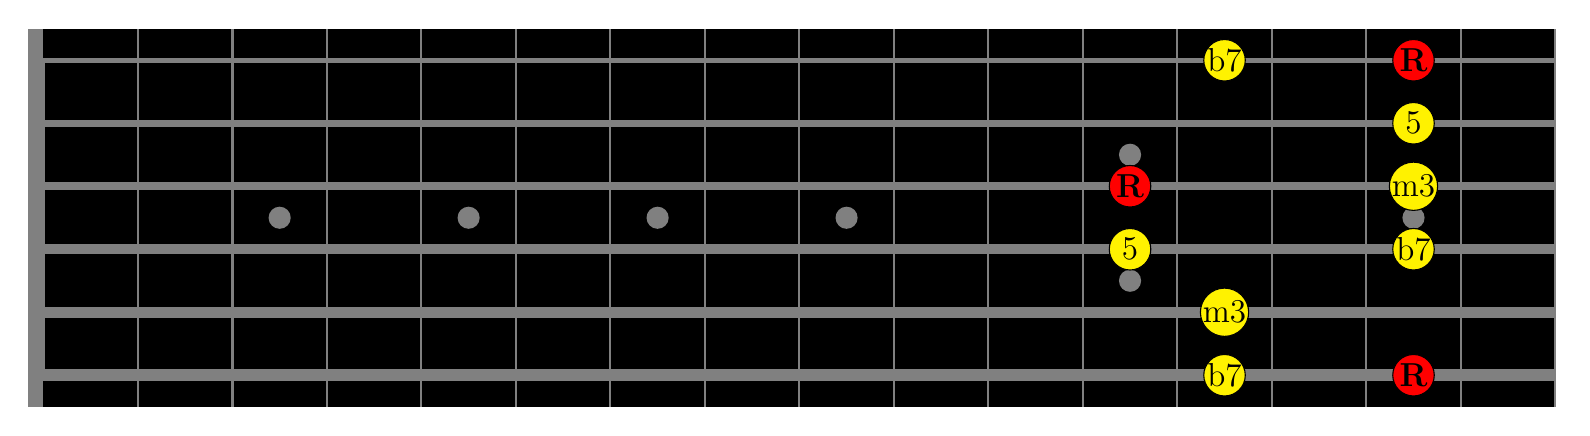
\begin{tikzpicture}[scale=1]
	\def \h{0.8}
	\def \fret{1.2} % 1.6
	\def \L{ 16*\fret }
	\def \dot_size{4pt}
	\def \circ_size{15pt}

	\fill[black, line width=2] (0.0,-0.4) rectangle (16*\fret,4.4);
	\fill[black!50!white, line width=2] (-0.2,-0.4) rectangle (0,4.4);

	% Strings
	\draw[color=black!50!white, line width=2.0]  (-0.1, 5*\h) -- (\L,5*\h); % E
	\draw[color=black!50!white, line width=2.5]  (-0.1, 4*\h) -- (\L,4*\h); % B
	\draw[color=black!50!white, line width=3.0]  (-0.1, 3*\h) -- (\L,3*\h); % G
	\draw[color=black!50!white, line width=3.5]  (-0.1, 2*\h) -- (\L,2*\h); % D
	\draw[color=black!50!white, line width=4.0]  (-0.1, 1*\h) -- (\L,1*\h); % A
	\draw[color=black!50!white, line width=4.5]  (-0.1, 0*\h) -- (\L,0*\h); % E

	% Frets 0
	\draw[color=black!50!white, thick]  (-0.1, 0) -- (-0.1,5*\h);
	\draw[color=black!50!white, thick]  (0, 0)   -- (0,5*\h);

	% Fret 1-15
	\draw[color=black!50!white, thick]  (\fret,   -0.4)   -- (\fret,4.4);
	\draw[color=black!50!white, thick]  (2*\fret, -0.4) -- (2*\fret,4.4);
	\draw[color=black!50!white, thick]  (3*\fret, -0.4) -- (3*\fret,4.4);
	\draw[color=black!50!white, thick]  (4*\fret, -0.4) -- (4*\fret,4.4);
	\draw[color=black!50!white, thick]  (5*\fret, -0.4) -- (5*\fret,4.4);
	\draw[color=black!50!white, thick]  (6*\fret, -0.4) -- (6*\fret,4.4);
	\draw[color=black!50!white, thick]  (7*\fret, -0.4) -- (7*\fret,4.4);
	\draw[color=black!50!white, thick]  (8*\fret, -0.4) -- (8*\fret,4.4);
	\draw[color=black!50!white, thick]  (9*\fret, -0.4) -- (9*\fret,4.4);
	\draw[color=black!50!white, thick]  (10*\fret, -0.4) -- (10*\fret,4.4);
	\draw[color=black!50!white, thick]  (11*\fret, -0.4) -- (11*\fret,4.4);
	\draw[color=black!50!white, thick]  (12*\fret, -0.4) -- (12*\fret,4.4);
	\draw[color=black!50!white, thick]  (13*\fret, -0.4) -- (13*\fret,4.4);
	\draw[color=black!50!white, thick]  (14*\fret, -0.4) -- (14*\fret,4.4);
	\draw[color=black!50!white, thick]  (15*\fret, -0.4) -- (15*\fret,4.4);
	\draw[color=black!50!white, thick]  (16*\fret, -0.4) -- (16*\fret,4.4);
	
	% Dots
	\fill[black!50!white] (2.5*\fret,2.5*\h) circle (\dot_size); % fret 3
	\fill[black!50!white] (4.5*\fret,2.5*\h) circle (\dot_size); % fret 5
	\fill[black!50!white] (6.5*\fret,2.5*\h) circle (\dot_size); % fret 7
	\fill[black!50!white] (8.5*\fret,2.5*\h) circle (\dot_size); % fret 9
	\fill[black!50!white] (11.5*\fret,1.5*\h) circle (\dot_size); % fret 12
	\fill[black!50!white] (11.5*\fret,3.5*\h) circle (\dot_size); % fret 12
	\fill[black!50!white] (14.5*\fret,2.5*\h) circle (\dot_size); % fret 15

	% Arpege (position G-E)
	\node[dot=\circ_size, fill=red,draw] at (14.5*\fret,0*\h) {{\large \textbf{R}}};
	\node[dot=\circ_size, fill=yellow,draw] at (12.5*\fret,0*\h) {{\large b7}};
	\node[dot=\circ_size, fill=yellow,draw] at (12.5*\fret,1*\h) {{\large m3}};
	\node[dot=\circ_size, fill=yellow,draw] at (11.5*\fret,2*\h) {{\large 5}};
	\node[dot=\circ_size, fill=yellow,draw] at (14.5*\fret,2*\h) {{\large b7}};
	\node[dot=\circ_size, fill=red,draw] at (11.5*\fret,3*\h) {{\large \textbf{R}}};
	\node[dot=\circ_size, fill=yellow,draw] at (14.5*\fret,3*\h) {{\large m3}};
	\node[dot=\circ_size, fill=yellow,draw] at (14.5*\fret,4*\h) {{\large 5}};
	\node[dot=\circ_size, fill=yellow,draw] at (12.5*\fret,5*\h) {{\large b7}};
	\node[dot=\circ_size, fill=red,draw] at (14.5*\fret,5*\h) {{\large \textbf{R}}};
%
%	% Annotation
%	\draw[black,anchor=west] (-3cm,2cm) node { {\Huge m7 } };
	
\end{tikzpicture}
%\end{document}




}

	\caption{(left) dom7 arpeggio. (right) m7 arpeggio. E-shape position, D-shape position, C-shape position, A-shape position, G-shape position (CAGED system)}
	\label{fig:arpeggio1}
\end{figure}


% Figure
\begin{figure}[!h]
	\hspace*{-4.2cm}
	\scalebox{0.52}{%\documentclass{standalone}
%\usepackage{pgfplots} % Include package for TikZ and PGF plot
%\usepackage{anyfontsize} % enable to change the font size manually
%\usepackage{makecell}%
%\usetikzlibrary{shapes.geometric}
%\tikzset{
%dot/.style = {circle, fill, minimum size=#1,
%              inner sep=0pt, outer sep=0pt},
%dot/.default = 6pt % size of the circle diameter
%}
% \renewcommand{\familydefault}{\sfdefault}

%\begin{document}
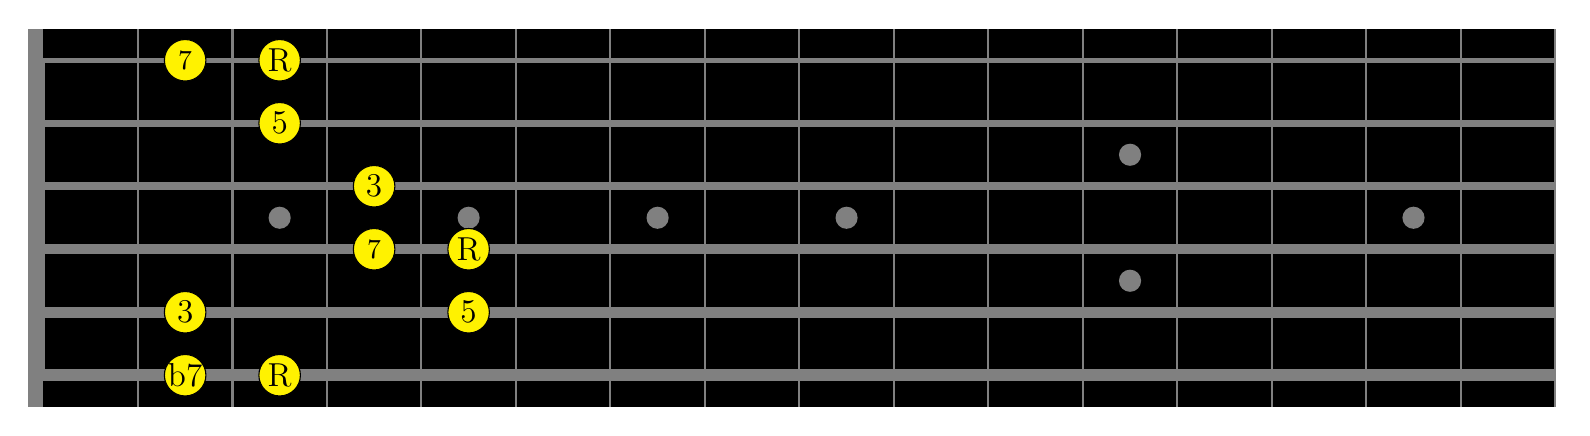
\begin{tikzpicture}[scale=1]
	\def \h{0.8}
	\def \fret{1.2} % 1.6
	\def \L{ 16*\fret }	
	\def \dot_size{4pt}
	\def \circ_size{15pt}
	
	\fill[black, line width=2] (0.0,-0.4) rectangle (16*\fret,4.4);
	\fill[black!50!white, line width=2] (-0.2,-0.4) rectangle (0,4.4);
	
	% Strings
	\draw[color=black!50!white, line width=2.0]  (-0.1, 5*\h) -- (\L,5*\h); % E
	\draw[color=black!50!white, line width=2.5]  (-0.1, 4*\h) -- (\L,4*\h); % B
	\draw[color=black!50!white, line width=3.0]  (-0.1, 3*\h) -- (\L,3*\h); % G
	\draw[color=black!50!white, line width=3.5]  (-0.1, 2*\h) -- (\L,2*\h); % D
	\draw[color=black!50!white, line width=4.0]  (-0.1, 1*\h) -- (\L,1*\h); % A
	\draw[color=black!50!white, line width=4.5]  (-0.1, 0*\h) -- (\L,0*\h); % E
	
	% Frets 0
	\draw[color=black!50!white, thick]  (-0.1, 0) -- (-0.1,5*\h); 
	\draw[color=black!50!white, thick]  (0, 0)   -- (0,5*\h); 
	
	% Fret 1-15
	\draw[color=black!50!white, thick]  (\fret,   -0.4)   -- (\fret,4.4);   
	\draw[color=black!50!white, thick]  (2*\fret, -0.4) -- (2*\fret,4.4); 
	\draw[color=black!50!white, thick]  (3*\fret, -0.4) -- (3*\fret,4.4); 
	\draw[color=black!50!white, thick]  (4*\fret, -0.4) -- (4*\fret,4.4); 
	\draw[color=black!50!white, thick]  (5*\fret, -0.4) -- (5*\fret,4.4); 
	\draw[color=black!50!white, thick]  (6*\fret, -0.4) -- (6*\fret,4.4); 
	\draw[color=black!50!white, thick]  (7*\fret, -0.4) -- (7*\fret,4.4); 
	\draw[color=black!50!white, thick]  (8*\fret, -0.4) -- (8*\fret,4.4); 
	\draw[color=black!50!white, thick]  (9*\fret, -0.4) -- (9*\fret,4.4); 
	\draw[color=black!50!white, thick]  (10*\fret, -0.4) -- (10*\fret,4.4); 
	\draw[color=black!50!white, thick]  (11*\fret, -0.4) -- (11*\fret,4.4); 
	\draw[color=black!50!white, thick]  (12*\fret, -0.4) -- (12*\fret,4.4); 
	\draw[color=black!50!white, thick]  (13*\fret, -0.4) -- (13*\fret,4.4); 
	\draw[color=black!50!white, thick]  (14*\fret, -0.4) -- (14*\fret,4.4); 
	\draw[color=black!50!white, thick]  (15*\fret, -0.4) -- (15*\fret,4.4); 
	\draw[color=black!50!white, thick]  (16*\fret, -0.4) -- (16*\fret,4.4); 
	%\draw[color=black!50!white, thick]  (17*\fret, -0.4) -- (17*\fret,4.4); 
	%\draw[color=black!50!white, thick]  (18*\fret, -0.4) -- (18*\fret,4.4); 
	%\draw[color=black!50!white, thick]  (19*\fret, -0.4) -- (19*\fret,4.4); 
	%\draw[color=black!50!white, thick]  (20*\fret, -0.4) -- (20*\fret,4.4); 
	
	% Dots
	\fill[black!50!white] (2.5*\fret,2.5*\h) circle (\dot_size); % fret 3
	\fill[black!50!white] (4.5*\fret,2.5*\h) circle (\dot_size); % fret 5
	\fill[black!50!white] (6.5*\fret,2.5*\h) circle (\dot_size); % fret 7
	\fill[black!50!white] (8.5*\fret,2.5*\h) circle (\dot_size); % fret 9
	\fill[black!50!white] (11.5*\fret,1.5*\h) circle (\dot_size); % fret 12
	\fill[black!50!white] (11.5*\fret,3.5*\h) circle (\dot_size); % fret 12
	\fill[black!50!white] (14.5*\fret,2.5*\h) circle (\dot_size); % fret 15
	%\fill[black!50!white] (16.5*\fret,2.5*\h) circle (\dot_size); % fret 17
	%\fill[black!50!white] (18.5*\fret,2.5*\h) circle (\dot_size); % fret 19

	
	% Arpege (position E)
	\node[dot=\circ_size, fill=yellow,draw] at (1.5*\fret,0) {{\large b7}};
	\node[dot=\circ_size, fill=yellow,draw] at (2.5*\fret,0) {{\large R}};
	\node[dot=\circ_size, fill=yellow,draw] at (1.5*\fret,1*\h) {{\large 3}};
	%\node[dot=\circ_size, fill=yellow,draw] at (1.5*\fret,1*\h) {{\large 3}};
	\node[dot=\circ_size, fill=yellow,draw] at (4.5*\fret,1*\h) {{\large 5}};
	\node[dot=\circ_size, fill=yellow,draw] at (3.5*\fret,2*\h) {{\normalsize 7}};
	\node[dot=\circ_size, fill=yellow,draw] at (4.5*\fret,2*\h) {{\large R}};
	\node[dot=\circ_size, fill=yellow,draw] at (3.5*\fret,3*\h) {{\large 3}};
	\node[dot=\circ_size, fill=yellow,draw] at (2.5*\fret,4*\h) {{\large 5}};
	\node[dot=\circ_size, fill=yellow,draw] at (1.5*\fret,5*\h) {{\normalsize 7}};
	\node[dot=\circ_size, fill=yellow,draw] at (2.5*\fret,5*\h) {{\large R}};
	
%	% Arpege (position D-C)
%	\node[dot=\circ_size, fill=white,draw] at (8.5*\fret,1*\h) {{\normalsize 7}};
%	\node[dot=\circ_size, fill=yellow!50!red!65!white,draw] at (9.5*\fret,1*\h) {{\large R}};
%	\node[dot=\circ_size, fill=yellow!50!red!30!white,draw] at (8.5*\fret,2*\h) {{\large 3}};
%	\node[dot=\circ_size, fill=yellow!50!red!30!white,draw] at (6.5*\fret,3*\h) {{\large 5}};
%	\node[dot=\circ_size, fill=white,draw] at (6.5*\fret,4*\h) {{\normalsize M7}};
%	\node[dot=\circ_size, fill=yellow!50!red!30!white,draw] at (7.5*\fret,4*\h) {{\large R}};
%	\node[dot=\circ_size, fill=yellow!100!red!50!white,draw] at (6.5*\fret,5*\h) {{\large 3}};
%	\node[dot=\circ_size, fill=yellow!50!red!65!white,draw] at (9.5*\fret,5*\h) {{\large 5}};
	
	% Arpege (position A)
%	\node[dot=\circ_size, fill=yellow!50!red!80!white,draw] at (13.5*\fret,1*\h) {{\large 3}};
%	\node[dot=\circ_size, fill=yellow!50!red!80!white,draw] at (11.5*\fret,2*\h) {{\large 5}};
%	\node[dot=\circ_size, fill=white,draw] at (10.5*\fret,3*\h) {{\normalsize M7}};
%	\node[dot=\circ_size, fill=yellow!50!red!80!white,draw] at (11.5*\fret,3*\h) {{\large R}};
%	\node[dot=\circ_size, fill=yellow!50!red!80!white,draw] at (11.5*\fret,4*\h) {{\large 3}};
%	\node[dot=\circ_size, fill=white,draw] at (13.5*\fret,5*\h) {{\normalsize M7}};
%	\node[dot=\circ_size, fill=yellow!50!red!80!white,draw] at (14.5*\fret,5*\h) {{\large R}};

%	% Annotation
%	\draw[black,anchor=west] (-3cm,2cm) node { {\Huge $\Delta$7 } };
	
\end{tikzpicture}
%\end{document}




}
	\hspace*{-0cm}
	\scalebox{0.52}{\input{figures/5.arpeges/m7b5/m7b5_pos1.tex}}

	\hspace*{-4.2cm}
	\scalebox{0.52}{\input{figures/5.arpeges/maj7/maj7_pos2.tex}}
	\hspace*{-0cm}
	\scalebox{0.52}{\input{figures/5.arpeges/m7b5/m7b5_pos2.tex}}

	\hspace*{-4.2cm}
	\scalebox{0.52}{\input{figures/5.arpeges/maj7/maj7_pos3.tex}}
	\hspace*{-0cm}
	\scalebox{0.52}{\input{figures/5.arpeges/m7b5/m7b5_pos3.tex}}

	\hspace*{-4.2cm}
	\scalebox{0.52}{\input{figures/5.arpeges/maj7/maj7_pos4.tex}}
	\hspace*{-0cm}
	\scalebox{0.52}{\input{figures/5.arpeges/m7b5/m7b5_pos4.tex}}

	\hspace*{-4.2cm}
	\scalebox{0.52}{\input{figures/5.arpeges/maj7/maj7_pos5.tex}}
	\hspace*{-0cm}
	\scalebox{0.52}{\input{figures/5.arpeges/m7b5/m7b5_pos5.tex}}

	\caption{(left) maj7 arpeggio (EDCAG). (right) m7b5 arpeggio}
	\label{fig:arpeggio2}
\end{figure}

%%%%%%%%%%%%%%%%%%%%%%%%%%%%%%%%%%%%%%%%%%%%%%%%%%%%%%%%%%%%%%%%%%%%%%%%%%%%%%%%%%%%%%%%%%%%%%%%%%%%%%%%%%%
\clearpage
\section{Blues}

\subsection{Blues scales}

% Table
\begin{table*}[!h]
	\caption{Blues scales (relative to the major scale)}
	\centering
	%\begin{adjustwidth}{0cm}{}
	\begin{tabular}{l|cccccccc}
		Scale name  & \multicolumn{8}{c}{Formula} \\
		\hline \hline \vspace{-0.4cm} \\
		Blues Major   & 1 & 2  & \textcolor{red}{b3} & 3  &   -   & 5  & 6  &  -  \\
		Blues minor   & 1 &  - & b3 & 4  & \textcolor{red}{b5} &  5  & - &  b7 \\
	\end{tabular}
	\label{tab: }
	%\end{adjustwidth}
\end{table*}


\begin{figure}[!h]
	\centering
	\hspace*{-1cm}
	\scalebox{0.7}{\input{figures/6.blues/gammes/blues_penta_mineur.tex}}
	\hspace*{-1cm}
	\scalebox{0.7}{
\renewcommand{\familydefault}{\sfdefault}

%\begin{document}
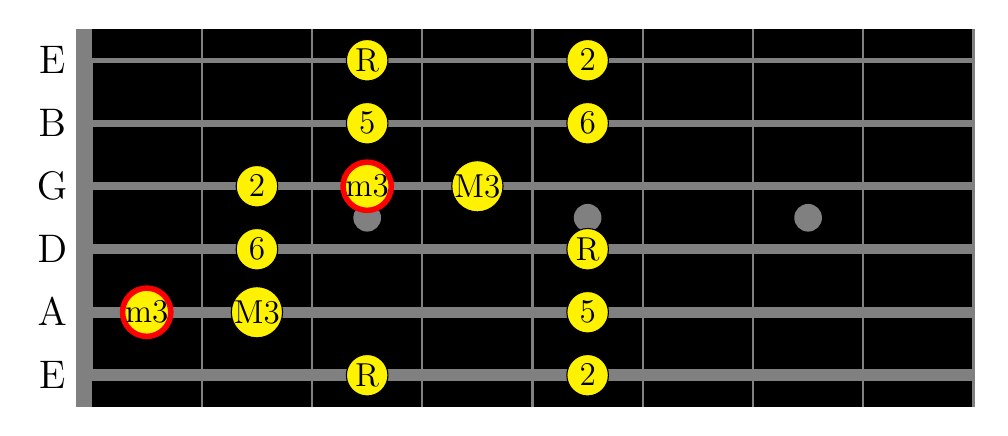
\begin{tikzpicture}[scale=1]
	\def \h{0.8}
	\def \fret{1.4} % 1.6
	\def \L{ 8*\fret }	
	\def \dot_size{5pt}
	\def \circ_size{15pt}
	
	\fill[black, line width=2] (0.0,-0.4) rectangle (8*\fret,4.4);
	\fill[black!50!white, line width=2] (-0.2,-0.4) rectangle (0,4.4);
	
	% Strings
	\draw[color=black!50!white, line width=2.0]  (-0.1, 5*\h) -- (\L,5*\h); % E
	\draw[color=black!50!white, line width=2.5]  (-0.1, 4*\h) -- (\L,4*\h); % B
	\draw[color=black!50!white, line width=3.0]  (-0.1, 3*\h) -- (\L,3*\h); % G
	\draw[color=black!50!white, line width=3.5]  (-0.1, 2*\h) -- (\L,2*\h); % D
	\draw[color=black!50!white, line width=4.0]  (-0.1, 1*\h) -- (\L,1*\h); % A
	\draw[color=black!50!white, line width=4.5]  (-0.1, 0*\h) -- (\L,0*\h); % E
	
	% Frets 0
	\draw[color=black!50!white, thick]  (-0.1, 0) -- (-0.1,5*\h); 
	\draw[color=black!50!white, thick]  (0, 0)   -- (0,5*\h); 
	
	% Fret 1-15
	\draw[color=black!50!white, thick]  (\fret,   -0.4)   -- (\fret,4.4);   
	\draw[color=black!50!white, thick]  (2*\fret, -0.4) -- (2*\fret,4.4); 
	\draw[color=black!50!white, thick]  (3*\fret, -0.4) -- (3*\fret,4.4); 
	\draw[color=black!50!white, thick]  (4*\fret, -0.4) -- (4*\fret,4.4); 
	\draw[color=black!50!white, thick]  (5*\fret, -0.4) -- (5*\fret,4.4); 
	\draw[color=black!50!white, thick]  (6*\fret, -0.4) -- (6*\fret,4.4); 
	\draw[color=black!50!white, thick]  (7*\fret, -0.4) -- (7*\fret,4.4); 
	\draw[color=black!50!white, thick]  (8*\fret, -0.4) -- (8*\fret,4.4);
	
	% Dots
	\fill[black!50!white] (2.5*\fret,2.5*\h) circle (\dot_size); % fret 3
	\fill[black!50!white] (4.5*\fret,2.5*\h) circle (\dot_size); % fret 5
	\fill[black!50!white] (6.5*\fret,2.5*\h) circle (\dot_size); % fret 7
	
	% String names
	\draw[black] (-0.5,5*\h) node { {\Large E} };
	\draw[black] (-0.5,4*\h) node { {\Large B} };
	\draw[black] (-0.5,3*\h) node { {\Large G} };
	\draw[black] (-0.5,2*\h) node { {\Large D} };
	\draw[black] (-0.5,1*\h) node { {\Large A} };
	\draw[black] (-0.5,0*\h) node { {\Large E} };
	
	% Major scale (fret 1-5)
	\node[dot=\circ_size, fill=yellow,draw] at (2.5*\fret,0) {{\large \textcolor{black}{R}}};    % Root
	\node[dot=\circ_size, fill=yellow, draw] at (4.5*\fret,0) {{\large 2}};
	\node[dot=\circ_size, fill=yellow,draw] at (1.5*\fret,1*\h) {{\large M3}};
	\node[dot=\circ_size, draw=red, line width=2, fill=yellow, draw] at (0.5*\fret,1*\h) {{\large m3}};
	\node[dot=\circ_size, fill=yellow,draw] at (4.5*\fret,1*\h) {{\large 5}};
	\node[dot=\circ_size, fill=yellow,draw] at (1.5*\fret,2*\h) {{\large 6}};
	\node[dot=\circ_size, fill=yellow,draw] at (4.5*\fret,2*\h) {{\large R}}; % Root
	\node[dot=\circ_size, fill=yellow,draw] at (1.5*\fret,3*\h) {{\large 2}};
	\node[dot=\circ_size, fill=yellow,draw] at (3.5*\fret,3*\h) {{\large M3}};
	\node[dot=\circ_size, draw=red, line width=2, fill=yellow, draw] at (2.5*\fret,3*\h) {{\large m3}};
	\node[dot=\circ_size, fill=yellow,draw] at (2.5*\fret,4*\h) {{\large 5}};
	\node[dot=\circ_size, fill=yellow,draw] at (4.5*\fret,4*\h) {{\large 6}};
	\node[dot=\circ_size, fill=yellow,draw] at (2.5*\fret,5*\h) {{\large R}};
	\node[dot=\circ_size, fill=yellow,draw] at (4.5*\fret,5*\h) {{\large 2}};

	
\end{tikzpicture}
%\end{document}









}
	\hspace*{-1cm}
	\scalebox{0.7}{\input{figures/6.blues/gammes/blues_mix_maj_min.tex}}
	\caption{(a) Minor blues scale with blue note (b5). (b) Major blues pentatonic scale. (c) Blues scale  }
	\label{fig:}
\end{figure}


\subsection{12-bar blues chord progression}

\begin{figure}[!h]
    \centering
	\hspace*{0cm}
	\scalebox{1.5}{
\begin{tabular}{| c | c | c | c |}
		\hline
		\phantom{x}I7\phantom{x} & \phantom{x}I7\phantom{x} & \phantom{x}I7\phantom{x} & \phantom{x}I7\phantom{x}  \\
		\hline
		\phantom{x}IV7\phantom{x} & \phantom{x}IV7\phantom{x} & \phantom{x}I7\phantom{x} & \phantom{x}I7\phantom{x}  \\
		\hline
		\phantom{x}V7\phantom{x} & \phantom{x}IV7\phantom{x} & \phantom{x}I7\phantom{x} & \phantom{x}I7\phantom{x}  \\
		\hline
\end{tabular}









}
	\scalebox{1.5}{

\begin{tabular}{| c | c | c | c |}
		\hline
		\phantom{x}i7\phantom{x} & \phantom{x}i7\phantom{x} & \phantom{x}i7\phantom{x} & \phantom{x}i7\phantom{x}  \\
		\hline
		\phantom{x}iv7\phantom{x} & \phantom{x}iv7\phantom{x} & \phantom{x}i7\phantom{x} & \phantom{x}i7\phantom{x}  \\
		\hline
		v7 or V7 & \phantom{x}iv7\phantom{x} & \phantom{x}i7\phantom{x} & \phantom{x}V7\phantom{x}  \\
		\hline
\end{tabular}




}
	\scalebox{1.5}{
\begin{tabular}{| c | c | c | c |}
		\hline
		\phantom{x}I7\phantom{x} & \phantom{x}IV7\phantom{x} & \phantom{x}I7\phantom{x} & \phantom{x}I7\phantom{x}  \\
		\hline
		\phantom{x}IV7\phantom{x} & \phantom{x}IV7\phantom{x} & \phantom{x}I7\phantom{x} & \phantom{x}VI7\phantom{x}  \\
		\hline
		\phantom{x}ii7\phantom{x} & \phantom{x}V7\phantom{x} & \phantom{x}I7\phantom{x}   & ii7 - V7  \\
		\hline
\end{tabular}




}
	\caption{(a) Basic Blues chord progression. (b) minor blues chord progression. (c) Basic Jazz Blues chord progression}
	\label{fig:}
\end{figure}


%\begin{figure*}[!h]
%	\centering
%	\begin{tabular}{| c | c | c | c |}
%		\hline
%		\phantom{x}I7\phantom{x} & \phantom{x}\textbf{IV7}\phantom{x} & \phantom{x}I7\phantom{x} & \phantom{x}I7\phantom{x}  \\
%		\hline
%		\phantom{x}IV7\phantom{x} & \phantom{x}IV7\phantom{x} & \phantom{x}I7\phantom{x} & \phantom{x}I7\phantom{x}  \\
%		\hline
%		\phantom{x}V7\phantom{x} & \phantom{x}IV7\phantom{x} & \phantom{x}I7 - \textbf{vi7} & \textbf{ii7} - V7\phantom{x}  \\
%		\hline
%	\end{tabular}
%	\caption{Basic 12 bar major blues with a \textit{quick change} and \textit{turnaroun}d}
%	\label{tab: }
%\end{figure*}



%%%%%%%%%%%%%%%%%%%%%%%%%%%%%%%%%%%%%%%%%%%%%%%%%%%%%%%%%%%%%%%%%%
\clearpage
\section{Modes}

\begin{itemize}
	\item Ionian (Joy), dorian(Jazz), phrygian(flamenco,doom), lydian (floaty,mystery) (ex: E.T., Jurassic Park, Back to the Future), mixo(blues)(ex: AC/DC), aeolian(sad)(ex: Losing my Religion), locrian(tension)(ex:Bjork Army of Me)
\end{itemize}

%%%%%%%%%%%%%%%%%%%%%%%%%%%%%%%%%%%%%%%%%%%%%%%%%%%%%%%%%%%%%%%%%%
\clearpage
\section{Transposition}

https://www.youtube.com/watch?v=Vxac3hHrxg8

%%%%%%%%%%%%%%%%%%%%%%%%%%%%%%%%%%%%%%%%%%%%%%%%%%%%%%%%%%%%%%%%%%
\clearpage
\section{Composition variation (Shred Master Scott)}

\begin{itemize}
	\item Pedal tone
	\item Inversion
	\item Voice leading
\end{itemize}

\newpage
\nocite{Lizzio2023}
\bibliographystyle{plain}
\bibliography{library.bib}

\end{document}
